\documentclass[a4paper,11pt,dvipdfmx]{jsarticle}


% 数式
\usepackage{amsmath,amsfonts}
\usepackage{bm}

% 画像
\usepackage[dvipdfmx]{graphicx}
\usepackage{framed}

% 図形
\usepackage{tikz}
\usepackage{circuitikz}
\usepackage[utf8]{inputenc}
\usepackage{geometry}
\geometry{margin=2cm}
\usetikzlibrary{shapes.geometric}
\usetikzlibrary {shapes.misc}

% ソースコード
\usepackage{listings,jlisting,color}
\lstset{
basicstyle={\ttfamily},
identifierstyle={\small},
commentstyle={\smallitshape},
keywordstyle={\small\bfseries},
ndkeywordstyle={\small},
stringstyle={\small\ttfamily},
frame={tb},
breaklines=true,
columns=[l]{fullflexible},
numbers=left,
xrightmargin=0zw,
xleftmargin=3zw,
numberstyle={\scriptsize},
stepnumber=1,
numbersep=1zw,
lineskip=-0.5ex
}
\renewcommand{\lstlistingname}{ソースコード}

\usepackage{booktabs}

\usepackage{pgfplots}
\pgfplotsset{compat=1.18} % 最新の互換性を指定


\begin{document}
\definecolor{shadecolor}{gray}{0.70}

\begin{titlepage}
\noindent
\vspace{4cm}
\begin{center}
\begin{LARGE}
組込システムI \\
第7回  課題 \\
\vspace{8cm}
提出日  2025/06/05 \\
学籍番号  21T2166D \\
名前  渡辺 大樹 \\
\end{LARGE}
\end{center}
\end{titlepage}
\setcounter{page}{1}

\section{課題}
本課題では、イベント検出と電圧比較回路を用いた組込システムの実装を行った。具体的には以下の2つの演習を実施した:

\begin{enumerate}
\item 演習(1):RPi.GPIOライブラリを用いたスイッチ入力のイベント検出システムの実装
\item 演習(3):CDS素子と電圧比較回路(LM339)を用いた光センサーシステムの実装
\end{enumerate}

これらの演習を通じて、ポーリング方式とイベント検出方式の違い、および電圧比較回路の動作原理について理解を深めることを目的とした。

\section{使用部品}
\subsection{演習(1)で使用した部品}
\begin{itemize}
\item Raspberry Pi 4B
\item タクトスイッチ(1個)
\item ブレッドボード
\item ジャンパー線
\end{itemize}

\subsection{演習(3)で使用した部品}
\begin{itemize}
\item Raspberry Pi 4B
\item CDS光センサー(1個)
\item LM339電圧比較器IC(1個)
\item LED(1個)
\item タクトスイッチ(1個)
\item 抵抗:6.8kΩ(1個)、1kΩ(1個)
\item 可変抵抗:10kΩ(1個)
\item ブレッドボード
\item ジャンパー線
\end{itemize}

\section{回路の説明}
\subsection{演習(1)の回路構成}
演習(1)では、GPIO21番ピンにタクトスイッチを接続した。スイッチの一端はGND、もう一端はGPIO21に接続し、内部プルアップ抵抗を有効にしてスイッチ入力を検出した。

\textbf{使用したRaspberry Piの端子:}
\begin{itemize}
\item GPIO21(Pin 40):スイッチ入力
\item GND(Pin 39):グランド接続
\end{itemize}

\subsection{演習(3)の回路構成}
演習(3)では、より複雑な回路を実装した。CDS素子と6.8kΩ抵抗による分圧回路の出力をLM339の非反転入力(IN+)に、10kΩ可変抵抗による分圧回路の出力を反転入力(IN-)に接続した。LM339の出力はオープンコレクタタイプのため、プルアップ抵抗を介してGPIO20に接続した。

\textbf{使用したRaspberry Piの端子:}
\begin{itemize}
\item GPIO16(Pin 36):LED制御出力
\item GPIO20(Pin 38):比較器出力入力
\item GPIO21(Pin 40):スイッチ入力
\item +3.3V(Pin 1):電源供給
\item GND(Pin 39):グランド接続
\end{itemize}

\section{回路図}
\begin{figure}[htbp]
\centering
\begin{circuitikz}[american, scale=1, every node/.style={scale=0.8}]

% Raspberry Pi 4B representation
\draw[thick] (0,0) rectangle (2.5,6);
\node at (1.25,6.3) {\textbf{Raspberry Pi 4B}};

% GPIO pins with labels
\node[anchor=east] at (0,5.5) {Pin 1};
\node[anchor=west] at (0.2,5.5) {+3.3V};
\node[anchor=east] at (0,4.5) {Pin 36};
\node[anchor=west] at (0.2,4.5) {GPIO16};
\node[anchor=east] at (0,4) {Pin 38};
\node[anchor=west] at (0.2,4) {GPIO20};
\node[anchor=east] at (0,3.5) {Pin 40};
\node[anchor=west] at (0.2,3.5) {GPIO21};
\node[anchor=east] at (0,0.5) {Pin 39};
\node[anchor=west] at (0.2,0.5) {GND};

% Power lines
\draw[red, thick] (2.5,5.5) -- (11.88,5.5);
\node[above] at (8,5.5) {+3.3V};
% GND line from Pin 39 at the bottom of Raspberry Pi
\draw[black, thick] (2.5,0.5) -- (11.88,0.5);
\node[below] at (8,0.5) {GND};

% Switch circuit (closest to Raspberry Pi)
\draw (2.5,3.5) to[short] (3.5,3.5);
\draw (3.5,3.5) to[push button, l=SW] (3.5,2);
\draw (3.5,2) -- (3.5,0.5);

% LED circuit (next to switch)
\draw (2.5,4.5) to[short] (5,4.5);
\draw (5,4.5) to[R, l=1k$\Omega$] (5,3);
\draw (5,3) to[led, l=LED] (5,1.5);
\draw (5,1.5) -- (5,0.5);

% CDS sensor and voltage divider (right side)
\draw (7,4) to[photoresistor, l=CDS] (7,5.5);
\draw (7,4) to[R, l=6.8k$\Omega$] (7,2.5);
\draw (7,5.5) -- (7,5.5);
\draw (7,2.5) -- (7,0.5);

% Variable resistor for reference voltage
\draw (9,3.5) to[vR, l=10k$\Omega$] (9,5.5);
\draw (9,3.5) -- (9,0.5);

% LM339 Comparator
\draw (11,3) node[op amp, anchor=+] (opamp) {};
\node[right] at (opamp.out) {OUT};
\node[above] at (opamp.up) {V+};
\node[below] at (opamp.down) {GND};

% Connections to LM339
\draw (7,3.79) -- (11,3.79);
\draw (9,3) -- (11,3);
\draw (opamp.up) -- (11.88,5.5);
\draw (opamp.down) -- (11.88,0.5);

% % Pull-up resistor and connection to GPIO20
% \draw (opamp.out) to[short] (12.5,3);
% \draw (12.5,3) to[R, l=10k$\Omega$] (12.5,5.5);
\draw (12.9,3.37) -- (12.9,4) -- (2.5,4);

\end{circuitikz}
\caption{演習(3)の回路図}
\label{fig:circuit}
\end{figure}

\section{アルゴリズムの説明}
\subsection{演習(1)のアルゴリズム}
演習(1)では、イベント検出を用いたスイッチ入力処理を実装した。アルゴリズムの流れは以下の通りである:

\begin{enumerate}
\item GPIO21を入力ピンとして設定し、内部プルアップ抵抗を有効化
\item 立ち下がりエッジでイベントを検出するよう設定
\item コールバック関数\texttt{checkSW}をイベント発生時に呼び出すよう登録
\item メインループでフラグ\texttt{s}を監視し、スイッチの状態を表示
\item チャタリング防止のため200msのbounce timeを設定
\end{enumerate}

この方式により、CPUがポーリングを行う必要がなく、効率的なスイッチ入力検出が可能となった。

\subsection{演習(3)のアルゴリズム}
演習(3)では、2つのイベント検出を同時に処理するシステムを実装した:

\begin{enumerate}
\item GPIO設定:
   \begin{itemize}
   \item GPIO16をLED制御用出力として設定
   \item GPIO20をCDS比較器出力用入力として設定(プルアップ有効)
   \item GPIO21をスイッチ用入力として設定(プルアップ有効)
   \end{itemize}
\item イベント検出設定:
   \begin{itemize}
   \item スイッチ(GPIO21)の立ち下がりエッジで\texttt{sw\_callback}を呼び出し
   \item CDS比較器(GPIO20)の立ち下がりエッジで\texttt{cds\_callback}を呼び出し
   \end{itemize}
\item 処理ロジック:
   \begin{itemize}
   \item 暗くなるとCDS比較器がLOWを出力し、LEDを点灯
   \item スイッチが押されるとLEDを消灯
   \item グローバル変数\texttt{led\_on}でLED状態を管理
   \end{itemize}
\end{enumerate}

\section{結果}
\subsection{演習(1)の結果}
演習(1)では、スイッチを押すたびに「SW on」、スイッチを離すと「SW off」がコンソールに1秒間隔で表示された。イベント検出により、スイッチの状態変化を即座に検知できることが確認された。bounceTime=200msの設定により、チャタリングによる誤検出も効果的に防止された。

従来のポーリング方式と比較して、CPU使用率の削減とリアルタイム性の向上が実現された。

\subsection{演習(3)の結果}
演習(3)では、以下の動作が正常に確認された:

\begin{enumerate}
\item CDS素子に光が当たっている状態では、比較器出力がHIGHとなりLEDは消灯状態を維持
\item CDS素子を手で覆い暗くすると、比較器出力がLOWとなり「暗さ検知:LED点灯」が表示されLEDが点灯
\item LED点灯中にスイッチを押すと、「SW押下:LED消灯」が表示されLEDが消灯
\item 可変抵抗を調整することで、光の閾値を変更可能であることを確認
\end{enumerate}

実装した回路では、オープンコレクタ出力に対するプルアップ抵抗の必要性と、適切なエッジ検出の重要性が実証された。

\begin{figure}[htbp]
\centering
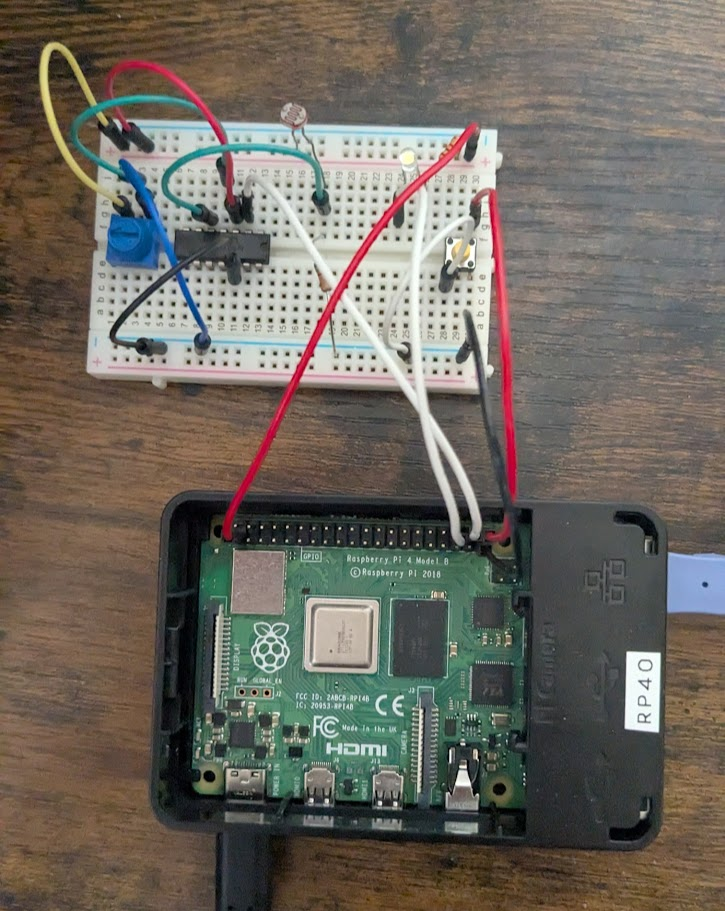
\includegraphics[width=0.8\textwidth]{image.png}
\caption{実装した回路の写真}
\label{fig:photo}
\end{figure}

\section{考察}
\subsection{イベント検出方式の優位性}
今回の実験を通じて、ポーリング方式とイベント検出方式の違いを実感できた。イベント検出方式では以下の利点が確認された:

\begin{itemize}
\item CPU使用率の削減:常時ポーリングが不要
\item リアルタイム性の向上:状態変化を即座に検知
\item 消費電力の削減:待機時の処理負荷軽減
\end{itemize}

特に組込システムにおいては、限られたリソースを効率的に活用する観点から、イベント駆動型の設計が重要であることが理解できた。

\subsection{電圧比較回路の応用}
LM339を用いた電圧比較回路は、アナログ信号をデジタル信号に変換する重要な役割を果たした。CDS素子による光強度の変化を電圧変化として捉え、閾値との比較によりデジタル判定を行うことで、マイコンでの処理が可能となった。

可変抵抗による閾値調整機能により、環境条件に応じた柔軟な設定が可能であることも確認できた。

\subsection{オープンコレクタ出力の特性}
LM339のオープンコレクタ出力特性により、プルアップ抵抗が必須であることを実験を通じて学んだ。この構成により、複数の出力をワイヤードOR接続することも可能であり、システム拡張性の観点でも有用な特性である。

\section{問いの解答}
\textbf{問い:オープンコレクタとはどの様なものか。}

\textbf{解答:}
オープンコレクタとは、トランジスタのコレクタが出力端子となっており、プルアップ抵抗を介して電源に接続する必要がある出力形式である。

具体的な動作は以下の通りである:
\begin{itemize}
\item \textbf{LOWレベル出力時:}内部のトランジスタがON状態となり、出力端子がGND(0V)に接続される
\item \textbf{HIGHレベル出力時:}内部のトランジスタがOFF状態となり、出力端子は外部のプルアップ抵抗を介して電源電圧まで引き上げられる
\end{itemize}

この構成の利点として、以下が挙げられる:
\begin{enumerate}
\item 複数の出力を並列接続(ワイヤードOR)可能
\item 異なる電源電圧レベルとのインターフェースが容易
\item 消費電力の削減が可能
\end{enumerate}

ただし、プルアップ抵抗が必須であり、これを忘れると正常な動作が得られないため注意が必要である。

% Python source codes
\newpage
\section{付録:ソースコード}
\subsection{演習(1)のソースコード}
\lstinputlisting[label=Python, caption=exam7-1.py]{C:/Program_Code/Python/BuiltIn/7/exam7-1.py}

\subsection{演習(3)のソースコード}
\lstinputlisting[label=Python2, caption=exam7-3.py]{C:/Program_Code/Python/BuiltIn/7/exam7-3.py}

\end{document}